\chapter{确定性推理}

\begin{question}
什么是图搜索过程?其中,重排OPEN表意味着什么?重排的原则是什么?
\end{question}	
\begin{solution}
图搜索的一般过程如下:
	\begin{enumerate}
		\item 建立一个只含有起始节点$S$的搜索图$G$,把$S$放到一个叫做OPEN的未扩展节点表中;
		\item 建立一个叫CLOSED的已扩展节点表,其初始为空表;
		\item LOOP:检查OPEN表是否为空,若为空,则失败退出;
		\item 选择OPEN表上的第一个节点,把它从OPEN表移出放进CLOSED表。并记该节点为节点$n$;
		\item 考察节点$n$是否为目标节点。若$n$为一目标节点,则有解并成功退出。此解是追踪图$G$中沿着指针从$n$到$S$这条路径而得到的(指针将在第7步中设置);
		\item 扩展节点$n$,生成一组子节点。把这些子节点中不是$n$的祖先的那些后继节点记入集合$M$。把$M$的这些成员作为$n$的后继节点添入图$G$中;
		\item 针对$M$中子节点的不同情况,分别作如下处理:
			\begin{itemize}
				\item 未曾在$G$中出现过的$M$成员设置一个通向其父节点(即节点$n$)的指针,并把$M$的这些成员加进OPEN表;(新生成的)
				\item 对已经在OPEN或CLOSED表上的每一个$M$成员,确定是否需要更改通到其父节点$n$的指针方向;(原生成但未扩展的)
				\item 对已在CLOSED表上的每个$M$成员,确定是否需要更改图$G$中通向它的每个后裔节点的指针方向;(原生成也扩展过的)
			\end{itemize}
		\item 按某一任意方式或按某个探试值,重排OPEN表;
		\item GO LOOP。
	\end{enumerate} \par
重排OPEN表意味着什么, 在第(6)步中,将优先扩展哪个节点,不同的排序标准对应着不同的搜索策略。是否重新安排OPEN表,即是否按照某个试探值(或准则、启发信息等)重新对未扩展节点进行排序,将决定该图搜索过程是无信息搜索或启发式搜索。各种搜索策略的主要区别在于对OPEN表中节点的排列顺序不同。例如,广度优先搜索把先生成的子节点排在前面,而深度优先搜索则把后生成的子节点排在前面。\par
重排的原则当视具体需求而定,不同的原则对应着不同的搜索策略,如果想尽快地找到一个解,则应当将最有可能达到目标节点的那些节点排在OPEN表的前面部分,如果想找到代价最小的解,则应当按代价从小到大的顺序重排OPEN表。
\end{solution}

\begin{question}
试举例比较各种搜索方法的效率。
\end{question}	
\begin{solution}
	\begin{description}
		\item[宽度优先搜索] 只要问题有解,用宽度优先搜索总可以得到解,而且得到的是路径最短的解。宽度优先搜索盲目性较大,当目标节点距初始节点较远时将会产生许多无用节点,搜索效率低。
		\item[深度优先搜索] 搜索一旦进入某个分支,就将沿着该分支一直向下搜索。如果目标节点恰好在此分支上,则可较快地得到解。但是,如果目标节点不在此分支上,而该分支又是一个无穷分支,则就不可能得到解。所以深度优先搜索是不完备的,即使问题有解,它也不一定能求得解。所求得的解答路径不一定是最短路径。
		\item[有界深度优先搜索] 如果问题有解,且其路径长度$\leq dm$,则搜索过程一定能求得解。但是,若解的路径长度$> dm$,则搜索过程就得不到解。这说明在有界深度优先搜索中,深度界限的选择是很重要的。要恰当地给出$dm$的值是比较困难的。即使能求出解,它也不一定是最优解。
		\item[等代价搜索] 是宽度优先搜索的一种推广,不是沿着等长度路径断层进行扩展,而是沿着等代价路径断层进行扩展。搜索树中每条连接弧线上的有关代价,表示时间、距离等花费。若所有连接弧线具有相等代价,则简化为宽度优先搜索算法。
		\item[盲目搜索] 具有较大的盲目性,产生的无用节点较多,效率不高,耗费过多的计算空间与时间。
		\item[有序搜索] 利用启发信息,决定哪个是下一步要扩展的节点。选``最有希望''的节点作为下一个被扩展的节点。选择OPEN表上具有最小$f$值的节点作为下一个要扩展的节点, 又称为最佳优先搜索。正确选择估价函数对搜索结果具有决定性的作用。使用不能识别某些节点真实希望的估价函数会形成非最小代价路径;使用一个过多地估计了全部节点希望的估价函数又会扩展过多的节点。 
		\item[A算法] 虽提高了算法效率,但不能保证找到最优解。
		\item[A*算法] 搜索效率很大程度上取决于估价函数$h(n)$。一般来说,在满足$h(n)\leq h^*(n)$的前提下,$h(n)$的值越大越好。$h(n)$的值越大,说明它携带的启发性信息越多,A*算法搜索时扩展的节点就越少,搜索效率就越高。
	\end{description}

\end{solution}

\begin{question}
化为子句型有哪些步骤?请结合例子说明。
\end{question}	
\begin{solution}
任一谓词演算公式可以化成一个子句集。其变换过程由下列九个步骤组成:
	\begin{enumerate}
		\item 消去蕴涵符号,将蕴涵符号化为析取和否定符号;
		\item 减少否定符号的辖域,每个否定符号最多只用到一个谓词符号上,并反复应用狄·摩根定律;
		\item 对变量标准化,对哑元改名,以保证每个量词有其自己唯一的哑元;
		\item 消去存在量词,引入Skolem函数,消去存在量词。如果要消去的存在量词不在任何一个全称量词的辖域内,那么我们就用不含变量的Skolem函数即常量;
		\item 化为前束形,把所有全称量词移到公式的左边,并使每个量词的辖域包括这个量词后面公式的整个部分;
		\item 把母式化为合取范式, 反复应用分配律,将母式写成许多合取项的合取的形式,而每一个合取项是一些谓词公式和(或)谓词公式的否定的析取;
		\item 消去全称量词,消去前缀,即消去明显出现的全称量词;
		\item 消去连词符号(合取),用{合取项1, 合取项2}替换明显出现的合取符号;
		\item 更换变量名称,更换变量符号的名称,使一个变量符号不出现在一个以上的子句中。
	\end{enumerate}
\end{solution}

\begin{question}
如何通过消解反演求取问题的答案。
\end{question}	
\begin{solution}
给出一个公式集$S$和目标公式$L$,通过反证或反演来求证目标公式$L$,其证明步骤如下: 
	\begin{enumerate}
		\item 否定$L$,得$\sim L$; 
		\item 把$\sim L$添加到$S$中去; 
		\item 把新产生的集合$\left\{\sim L, S\right\}$化成子句集; 
		\item 应用消解原理,力图推导出一个表示矛盾的空子句。
	\end{enumerate}
\end{solution}

\begin{question}
什么叫合式公式?合式公式有哪些等价关系?
\end{question}	
\begin{solution}
合式公式的递归定义如下:
	\begin{enumerate}
		\item 原子谓词公式是合式公式。
		\item 若$A$为合式公式,则$\sim A$也是一个合式公式。
		\item 若$A$、$B$是合式公式,则$A \vee B$,$A \wedge B$、$A \to B$、$A \leftrightarrow B$也都是合式公式。
		\item 若$A$是合式公式,$x$为$A$中的自由变量,则$\left(\forall x\right) A$和$\left(\exists x\right) A$都是合式公式。
		\item 运用有限步上述规则(1)至(4)求得的那些公式是是合式公式。
	\end{enumerate}
等价关系有:
	\begin{enumerate}
		\item 否定之否定:$\sim(\sim P)=P$
		\item 蕴含与与或形式的等价:$\begin{cases}
		P\to Q = \sim P \vee Q\\
		\sim P\to Q = P \vee Q
		\end{cases}$ 
		\item 狄•摩根定律:$\begin{cases}
		\sim (P \vee Q) = \sim P \wedge \sim Q \\
		\sim (P \wedge Q) = \sim P \vee \sim Q 
		\end{cases}$
		\item 分配律:$\begin{cases}
		P \vee (Q \wedge R) = (P \vee Q) \wedge (P \vee R) \\
		P \wedge (Q \vee R) = (P \wedge Q) \vee (P \wedge R)
		\end{cases}$
		\item 交换律:$\begin{cases}
		P \vee Q = Q \vee P \\
		P \wedge Q = Q \wedge P
		\end{cases}$
		\item 结合律:$\begin{cases}
		P \vee (Q \vee R) = (P \vee Q) \vee R \\
		P \wedge (Q \wedge R) = (P \wedge Q) \wedge R
		\end{cases}$
		\item 逆否率:$(P \to Q) = (\sim Q \to \sim P)$
		\item 否定跨越量词:$\sim (\exists x) P(x) = (\forall x)[\sim P(x)]$
		\item 全称量词同与或连词:$\begin{cases}
		(\forall x)[P(x) \wedge Q(x)] = (\forall x) P(x) \wedge (\forall x) Q(x) \\
		(\forall x)[P(x) \vee Q(x)] = (\forall x) P(x) \vee (\forall x) Q(x)
		\end{cases}$
		\item 量词中的哑元:$\begin{cases}
		(\forall x) P(x) = (\forall y) P(y) \\
		(\exists x) P(x) = (\exists y) P(y)
		\end{cases}$
	\end{enumerate}
\end{solution}

\begin{question}
用宽度优先搜索求图\ref{Fig:maze}所示迷宫的出路。
	\begin{figure}[h]
		\centering
		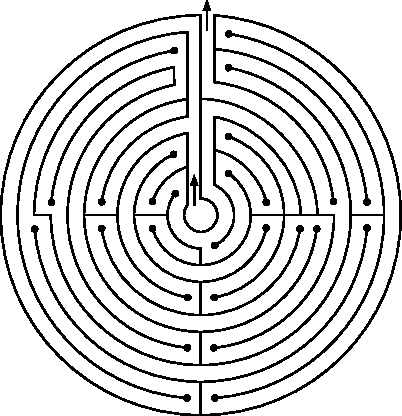
\includegraphics{figures/ques-3.6.pdf}
		\caption{迷宫一例} \label{Fig:maze}
	\end{figure}
\end{question}
\begin{solution}
\end{solution}

\begin{question}
用有界深度优先搜索方法求解图\ref{Fig:8-code}所示八数码难题。
	\begin{figure}[h]
		\centering
		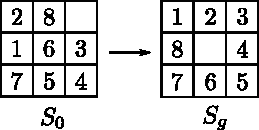
\includegraphics{figures/ques-3.7.pdf}
		\caption{八数码难题} \label{Fig:8-code}
	\end{figure}
\end{question}
\begin{solution}
\end{solution}

\begin{question}
应用最新的方法表达传教士和野人问题,编写一个计算机程序,以求得安全渡过全部$6$个人的解答。(提示:在应用状态空间表示和搜索方法时,可用$(N_m,N_c)$来表示状态描述,其中$N_m$和$N_c$分别为传教士和野人的人数。初始状态为$(3,3)$,而可能的中间状态为$(0,1)$,$(0,2)$,$(0,3)$,$(1,1)$,$(2,1)$,$(2,2)$,$(3,0)$,$(3,1)$和$(3,2)$等。
\end{question}
\begin{solution}
\end{solution}

\begin{question}
试比较宽度优先搜索、有界深度优先搜索及有序搜索的搜索效率,并以实例数据加以说明。
\end{question}
\begin{solution}
\end{solution}

\begin{question}
一个机器人驾驶卡车,携带包裹(编号分别为\#1、\#2和\#3)分别投递到林(LIN)、吴(WU)和胡(HU) 3家住宅处。规定了某些简单的操作符,如表示驾驶方位的$\mathrm{drive}(x,y)$和表示卸下包裹的$\mathrm{unload}(z)$;对于每个操作符,都有一定的先决条件和结果。试说明状态空间问题求解系统如何能够应用谓词演算求得一个操作符序列,该序列能够生成一个满足$\mathrm{AT(\# 1,LIN) \wedge AT(\# 2,WU) \wedge AT(\# 3,HU)}$的目标状态。
\end{question}
\begin{solution}
初始状态可描述为:
	\begin{multline*}
	\mathrm{AT}(\#1, \sim \mathrm{LIN}) \wedge \mathrm{AT}(\#2, \sim \mathrm{WU}) \wedge \mathrm{AT}(\#3, \sim \mathrm{HU}) \wedge {} \\
	\mathrm{AT}(\#1, \mathrm{CAR}) \wedge \mathrm{AT}(\#2, \mathrm{CAR}) \wedge \mathrm{AT}(\#3, \mathrm{CAR})
	\end{multline*} 
目标状态可描述为:
	\begin{multline*}
	\mathrm{AT}(\#1, \mathrm{LIN}) \wedge \mathrm{AT}(\#2, \mathrm{WU}) \wedge \mathrm{AT}(\#3, \mathrm{HU}) \wedge {} \\
	\mathrm{AT}(\#1, \sim \mathrm{CAR}) \wedge \mathrm{AT}(\#2, \sim \mathrm{CAR}) \wedge \mathrm{AT}(\#3, \sim \mathrm{CAR})
	\end{multline*}
对每个操作符都有一定的先决条件和结果,如表\ref{tab:operators}:
	\begin{table}[htbp]
	\centering
	\begin{tabular}{p{50pt}p{130pt}p{130pt}}
		\toprule
		~ & 先决条件 & 结果 \\
		\midrule
		$\mathrm{drive}(x,y)$ & $\mathrm{AT}(\mathrm{CAR}, x)$ & $\mathrm{AT}(\mathrm{CAR}, y)$ \\
		\midrule
		$\mathrm{unload}(z)$ & $\mathrm{AT}(z, \mathrm{CAR}) \wedge \mathrm{AT}(\mathrm{CAR}, x)$ 
			& $\mathrm{AT}(z, \sim\mathrm{CAR}) \wedge \mathrm{AT}(x, x)$ \\
		\bottomrule
	\end{tabular}
	\caption{每个操作符的先决条件和结果}\label{tab:operators}
	\end{table} \par
至此,原问题就转换为:寻找一个可将初始状态转换到目标状态的操作序列,如何求得该操作序列。
\end{solution}

\begin{question}
规则演绎系统和产生式系统有哪几种推理方式?各自的特点为是什么?
\end{question}
\begin{solution}
规则演绎系统的推理方式有正向推理、逆向推理和双向推理。正向推理、逆向推理的特点见表\ref{tab:reasoning-of-rule-based-system};双向推理组合了正向推理和逆向推理的优点,克服了各自的缺点,具有更高的搜索求解效率。
	\begin{table}[htbp]
	\centering
	\begin{tabular}{p{80pt}p{110pt}p{110pt}}
		\toprule
		~ & 正向推理 & 逆向推理 \\
		\midrule
		推理方向 & 从if部分向then部分推理的过程,它是从事实或状况向目标或动作进行操作的 & 从then部分向if部分推理的过程,它是从目标或动作向事实或状况进行操作的 \\
		\midrule
		目标表达式 & 文字的析取 & 任意形式 \\
		\midrule
		事实表达式 & 任意形式 & 文字的合取 \\
		\bottomrule
	\end{tabular}
	\caption{规则演绎系统系统的推理方式}\label{tab:reasoning-of-rule-based-system}
	\end{table} 
	\par
产生式系统的推理方式有正向推理、逆向推理和双向推理。正向推理、逆向推理的特点见表\ref{tab:reasoning-of-production-system};双向推理结合了正向推理和逆向推理的长处,克服了两者的短处,其控制策略比两者都要复杂。
	\begin{table}[htbp]
	\centering
	\begin{tabular}{p{80pt}p{110pt}p{110pt}}
		\toprule
		~ & 正向推理 & 逆向推理 \\
		\midrule
		驱动方式 & 数据驱动 & 目标驱动 \\ 
		\midrule
		推理方法 & 从一组数据出发向前推到结论 & 从可能的解答出发,向后推理验证解答 \\ 
		\midrule
		启动方法 & 从一个事件启动 & 由询问关于目标状态的一个问题而启动 \\ 
		\midrule
		透明程度 & 不能解释其推理过程 & 可解释其推理过程 \\ 
		\midrule
		推理方向 & 由底向上推理 & 由顶向下推理 \\ 
		\midrule
		优点 & 算法简单、容易实现,允许用户一开始就把有关的事实数据存入数据库,在执行过程中系统能很快获得这些数据,而不必等到系统需要数据时才向用户询问 & 搜索目的性强,推理效率高 \\ 
		\midrule
		缺点 & 盲目搜索,可能会求解许多与总目标无关的子目标,每当总数据库内容更新后都要遍历整个规则库,推理效率较低 & 目标的选择具有盲目性,可能会求解许多假的目标;当可能的结论数目很多,即目标空间很大时,推理效率不高;当规则的右部是执行某种动作不是结论时,逆向推理不便使用 \\ 
		\midrule
		适用场合 & 主要用于已知初始数据,而无法提供推理目标,或解空间很大的一类问题,如监控、预测、规划、设计等问题的求解 & 主要用于结论单一或者已知目标结论,而要求验证的系统,如选择、分类、故障诊断等问题的求解 \\ 
		\midrule
		典型系统 & CLIPS,OPS & PROLOG \\
		\bottomrule
	\end{tabular}
	\caption{产生式系统的推理方式}\label{tab:reasoning-of-production-system}
	\end{table}
\end{solution}

\begin{question}
单调推理有何局限性?什么叫缺省推理?非单调推理系统如何证实一个节点的有效性?
\end{question}
\begin{solution}
单调系统不能很好地处理常常出现在现实问题领域中的3类情况,即不完全的信息、不断变化的情况、以及求解复杂问题过程中生成的假设。有两种方法可以证实节点的有效性:
	\begin{enumerate}
		\item 支持表。(SL (IN-节点表) (OUT-节点表)) \\
			如果某节点的IN节点表中提到的节点当前都是IN, 且OUT节点表中提到的节点当前都是OUT,则它是有效的。
		\item 条件证明。(CP(结论) (IN-假设) (OUT-假设)) \\
			条件证明(CP)的证实表示有前提的论点,无论何时,只要在IN假设中的节点为IN,OUT假设中的节点为OUT,则结论节点往往为IN,于是条件证明的证实有效。 
	\end{enumerate}
\end{solution}

\begin{question}
在什么情况下需要采用不确定推理或非单调推理?
\end{question}
\begin{solution}
不完全的信息、不断变化的情况、以及求解复杂问题过程中生成的假设。
\end{solution}

\begin{question}
下列语句是一些几何定理,把这些语句表示为基于规则的几何证明系统的产生式规则:
	\begin{enumerate}
		\item 两个全等三角形的各对应角相等。
		\item 两个全等三角形的各对应边相等。 
		\item 各对应边相等的三角形是全等三角形。
		\item 等腰三角形的两底角相等。 
	\end{enumerate}
\end{question}
\begin{solution}
产生式规则如下:
	\begin{enumerate}
		\item IF 两个三角形全等 THEN 各对应角相等 
		\item IF 两个三角形全等 THEN 各对应边相等 
		\item IF 两个三角形各对应边相等 THEN 两三角形全等 
		\item IF 它是等腰三角形 THEN 它的两底角相等
	\end{enumerate}
\end{solution}